\section{Grundläggande koncept}

\paragraph{Syftet med reglerteknik}
Reglerteknik handlar om att kontrollera olika storheter, ofta betecknad $y$, i ett system mot något värde, ofta betecknad $r$. I tillägg till systemets egna beteende påverkas storheten vi vill reglera typiskt av en yttre störning $v$. Vi kan reglera systemet genom att tillföra en påverkan, ofta betecknad $u$.

\paragraph{Strategi}
För att förstå systemet, tar vi först fram en modell som beskriver det. Ur denna modellen fås typiskt en differentialekvation. Denna löser vi med Laplacetransform över tid.

\paragraph{Överförningsfungktionen}
För linjära system fås en lösning i Laplacerummet på formen $Y(s) = G(s)U(s)$, där $U$ är Laplacetransformen av $u$. Funktionen $G$ är överförningsfunktionen. Notera att denna lösningsformen typiskt beror på att alla initialvärden är $0$.

\paragraph{Poler}
Ett systems poler är rötterna till nämnarpolynomet (som typiskt finns) i överförningsfunktionen.

\paragraph{Stabilitet}
Ett system är stabilt om det tenderar mot ett visst läge efter lång tid. Systemets stabilitet är typiskt kopplad med dets poler. Detta kan man se i enkla fall, till exempel vanliga linjära ordinära differentialekvationer. Här är systemet stabilt om det inte finns några poler i högre halvplan, och avståndet längs med reella axeln anger hur snabbt lösningen tenderar mot det stabila läget.

\paragraph{Nollställen}
Ett systems nollställen är rötterna till täljarpolynomet (som typiskt finns) hos överförningsfunktioner. Eftersom vi är intresserade av att styra $y$, är det viktigt hur vi ska välja $u$ för att få det. Därmed är $\frac{1}{G}$ en viktig storhet, och nollställen kan därmed orsaka reglerproblem som är svårlösta.

\paragraph{Impulssvar}
Om lösningen för $Y$ är på formen $Y = GU$, är lösningen för $y$ på formen
\begin{align*}
	y(t) = \integ{0}{t}{\tau}{g(\tau)u(t - \tau)}.
\end{align*}
$g$ kallas för impulssvaret.

\paragraph{Blockschema}
Ett blockschema är ett systematisk sätt att rita reglerade system på. För att förstå hur man läser dem, betrakta figur \ref{fig:basic_block}.
\begin{figure}[!ht]
	\centering
	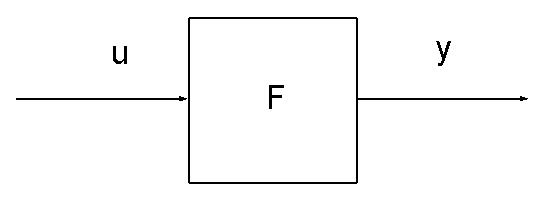
\includegraphics[width = 0.5\textwidth]{./Images/basic_block.eps}
	\caption{Illustration av ett enkelt blockschema.}
	\label{fig:basic_block}
\end{figure}

Med denna figuren menas att $Y(s) = F(s)U(s)$.

\paragraph{Rotort}
En rotort är en plott av ett systems poler som funktion av någon parameter. Den är typiskt uppdelad i grenar, som är kurvor i planet som är parametriserade av parametervärdet. Polerna som motsvarar parametervärdet $0$ är rotortens startpunkter, och polarna motsvarande parametervärdet $\infty$ är rotortens ändpunkter. Om rotorten närmar sig kurvor, är dessa rotortens asymptoter.